
%----------------------------------------------------------------------------
\chapter{Preliminaries}
%----------------------------------------------------------------------------



\section{Modeling using graphs}

Structural or behavioral modeling of systems are often done using graphs. .... \TODO{...}

\section{Runtime modeling}

In this thesis we use structural modeling to model the current state of the system. This model is called the live model, which captures the state and the operating context of the system.

\subsection{Runtime modeling example}



\section{Graph pattern matching concepts}

\begin{figure}[h]
	\begin{center}
		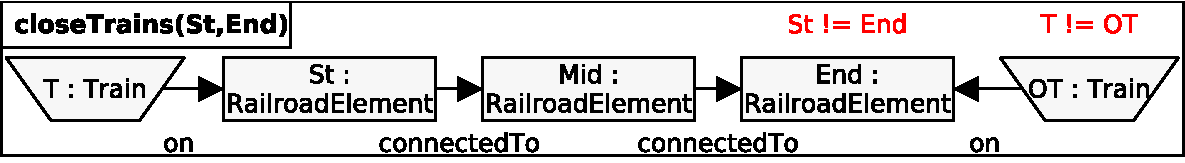
\includegraphics[width=0.75\textwidth]{figures/pattern-visual.pdf}
		\caption{Visual representation of a graph pattern}
		\label{pattern-visual}
	\end{center}
\end{figure}

A graph pattern's purpose is to define a set of constraints that can be satisfied by the vertices of the graph.

\section{Local search}
\todo{ezt kidolgozni}


Local search is an algorithm to provide matchings of a graph pattern in a graph.

\section{Distributed platform}

% adatok diszjunkt halmazokra bontva különböző csomópontra
% az algoritmusok is elosztottak, nem lesz összegyűjtve az infó, úgy van kiértékelve, hogy nincs aki mindent látna a rendszerből


